\chapter{Comparative sui risultati ottenuti}

\section{Matrici d'importanza}
\subsection{Dati Udine}
\begin{figure}
    \begin{center}
    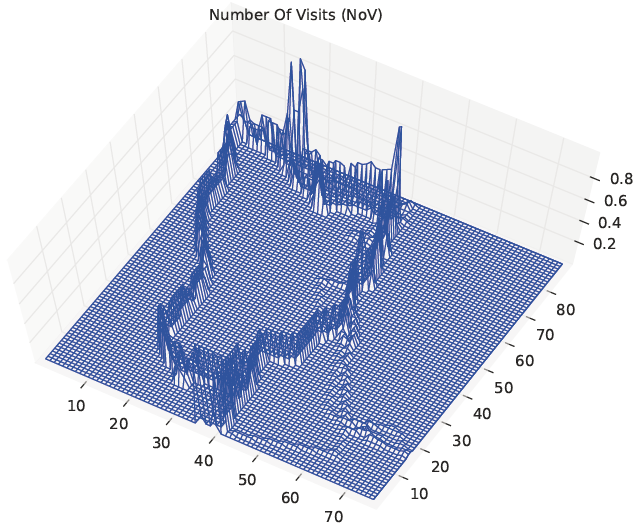
\includegraphics[scale=0.3]{Python/Python_Udine_NV.png}
    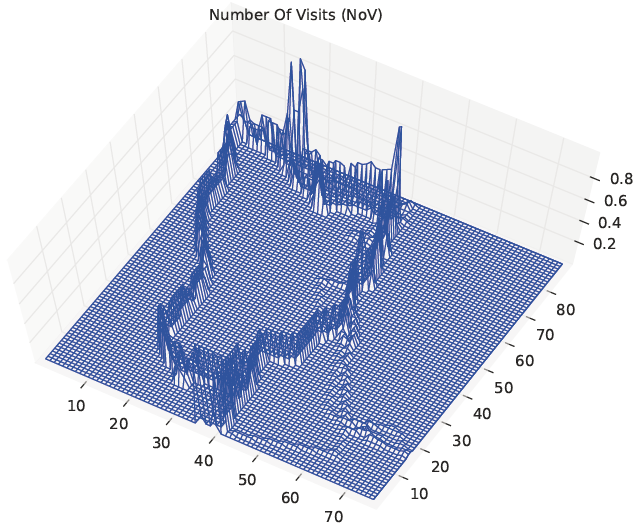
\includegraphics[scale=0.3]{Python/Python_Udine_NV.png}
    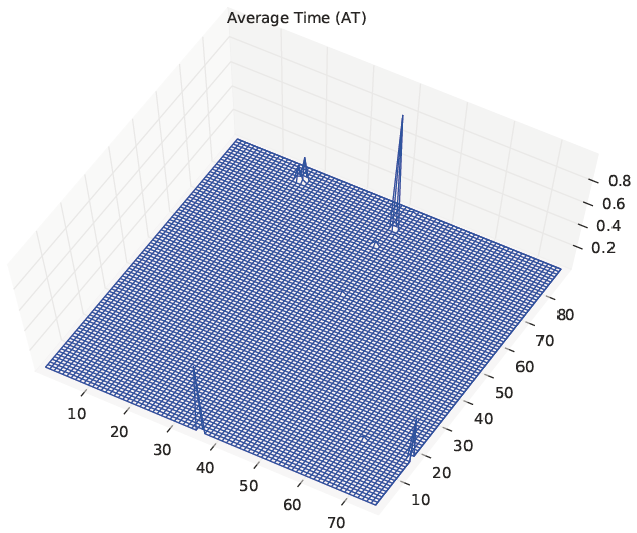
\includegraphics[scale=0.3]{Python/Python_Udine_AV.png}
    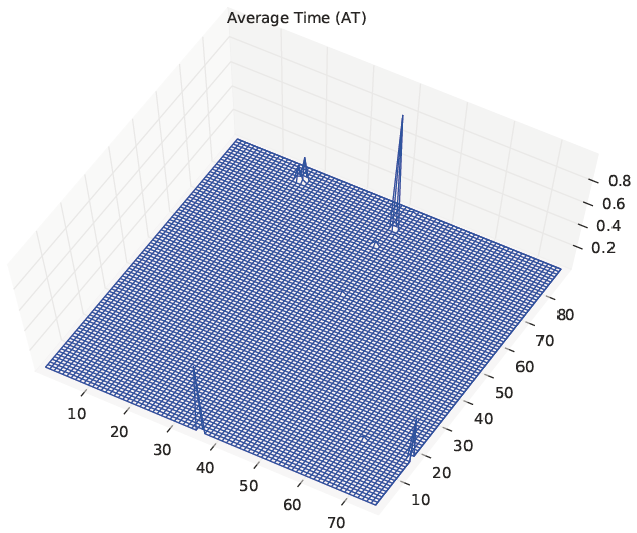
\includegraphics[scale=0.3]{Python/Python_Udine_AV.png}
    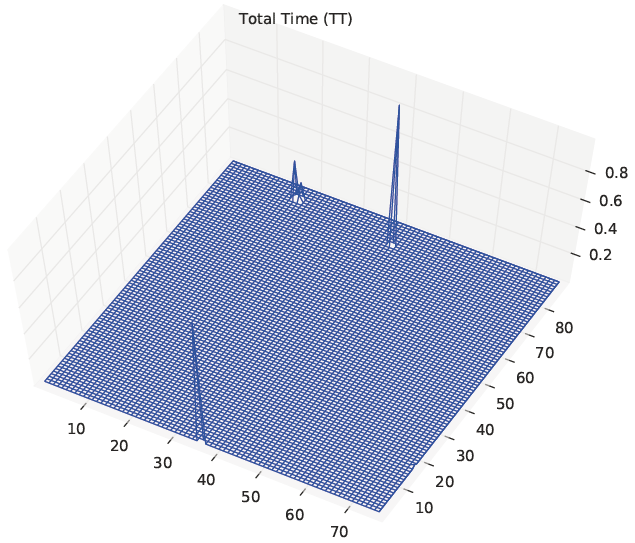
\includegraphics[scale=0.3]{Python/Python_Udine_TT.png}
    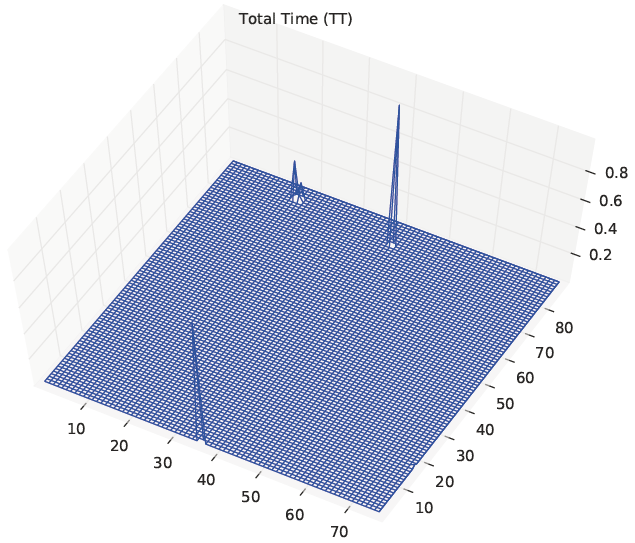
\includegraphics[scale=0.3]{Python/Python_Udine_TT.png}
    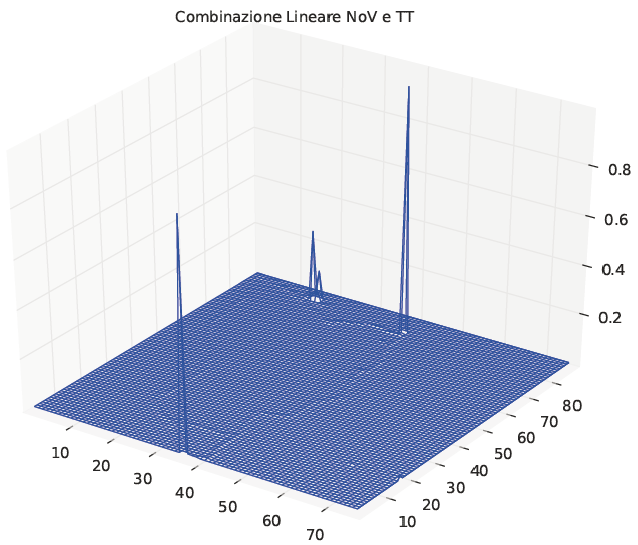
\includegraphics[scale=0.3]{Python/Python_Udine_CL.png}
    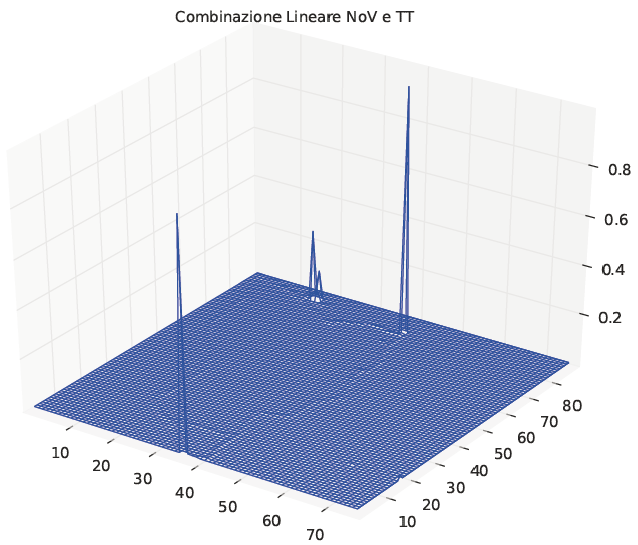
\includegraphics[scale=0.3]{Python/Python_Udine_CL.png}
    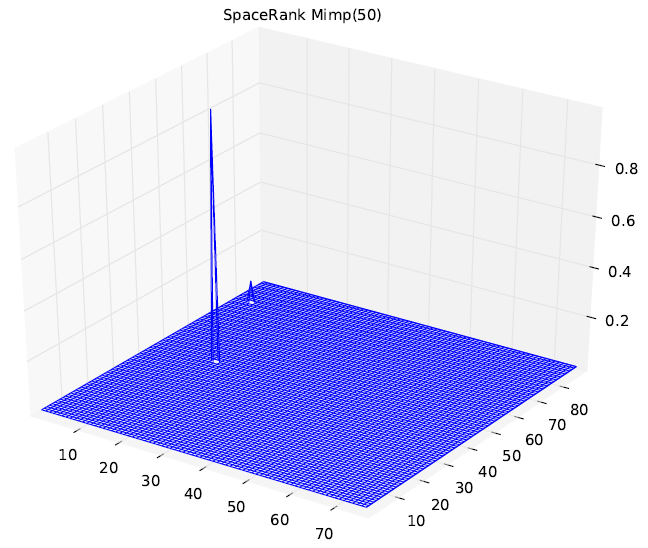
\includegraphics[scale=0.3]{Python/Python_Udine_SR.png}
    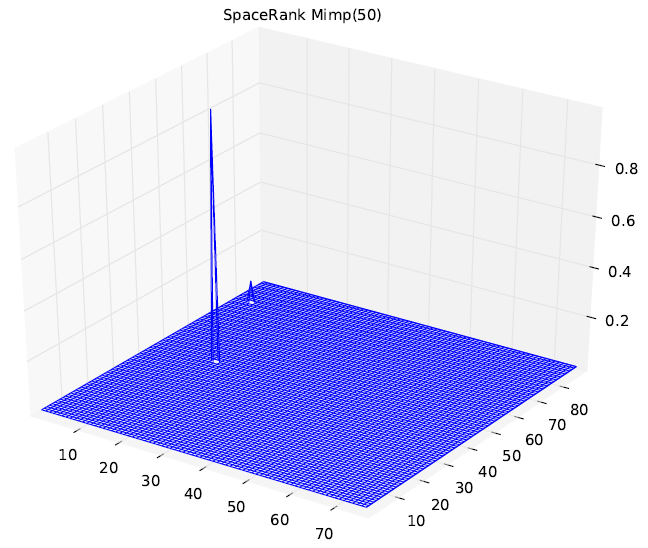
\includegraphics[scale=0.3]{Python/Python_Udine_SR.png}
    \caption[Arda 1]{Esempio di attrazione gravitazionale}
    \label{etichetta}
    \end{center}
\end{figure}
\subsection{Dati Atlanta}
\begin{figure}
    \begin{center}
    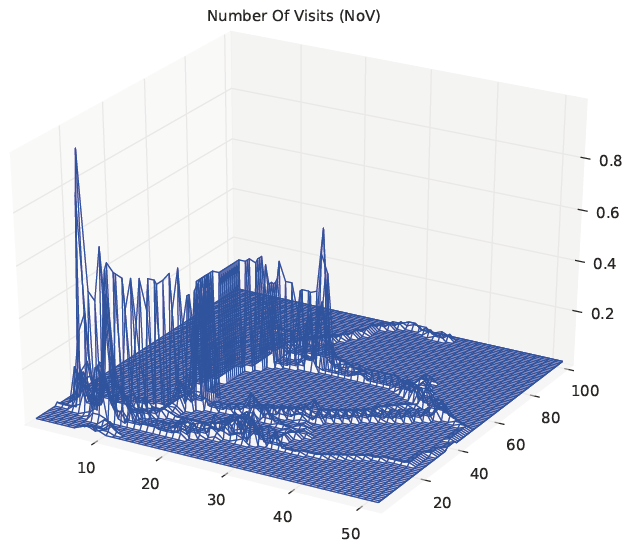
\includegraphics[scale=0.3]{Python/Python_Atlanta_NV.png}
    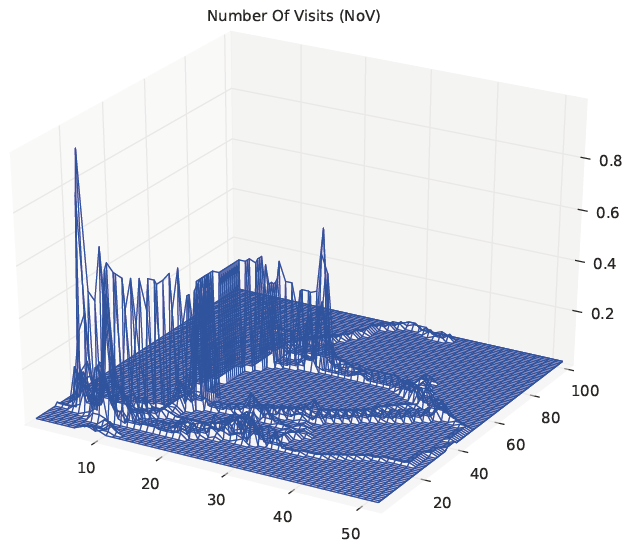
\includegraphics[scale=0.3]{Python/Python_Atlanta_NV.png}
    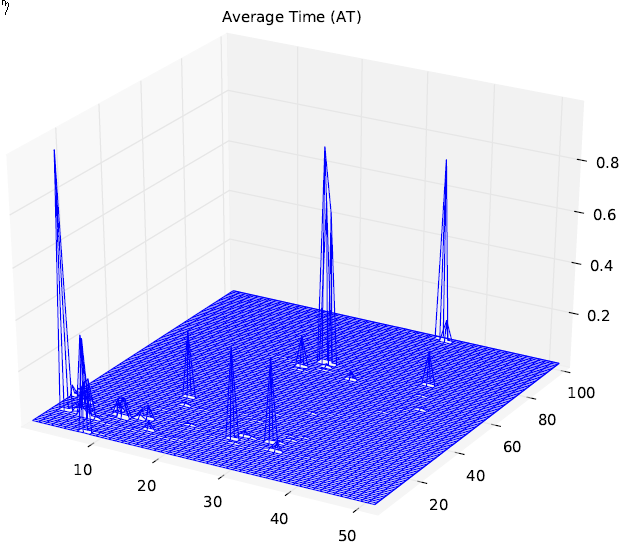
\includegraphics[scale=0.3]{Python/Python_Atlanta_AV.png}
    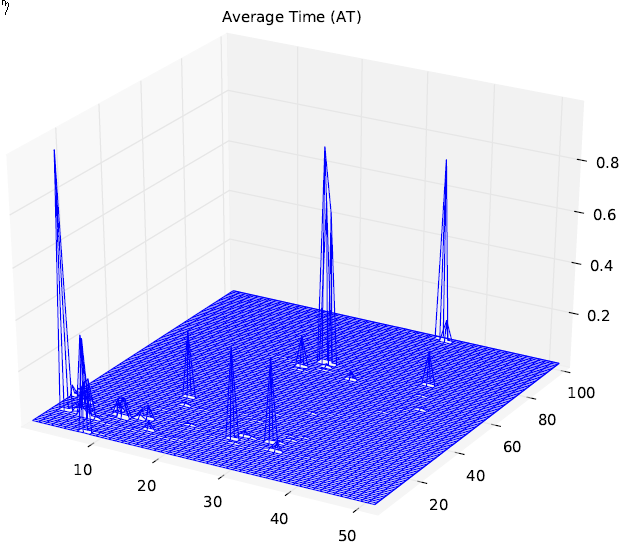
\includegraphics[scale=0.3]{Python/Python_Atlanta_AV.png}
    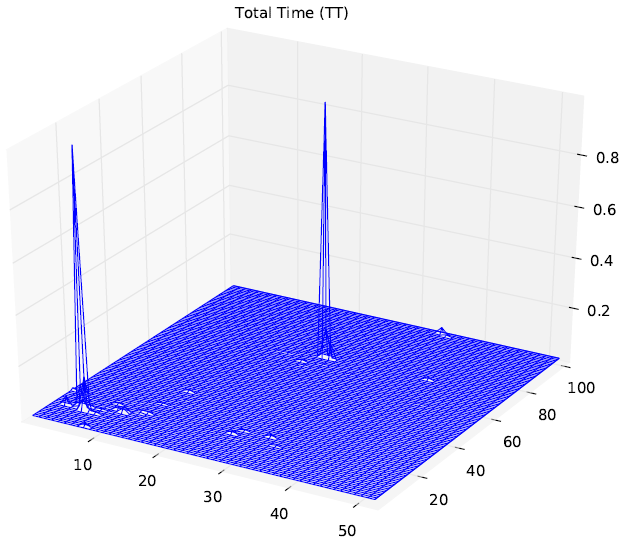
\includegraphics[scale=0.3]{Python/Python_Atlanta_TT.png}
    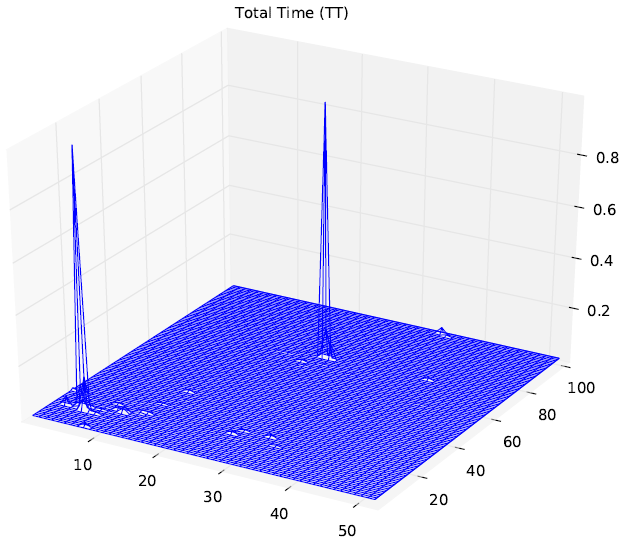
\includegraphics[scale=0.3]{Python/Python_Atlanta_TT.png}
    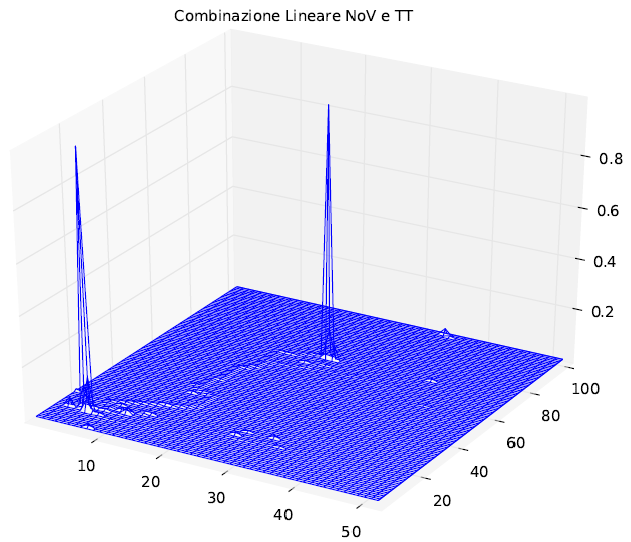
\includegraphics[scale=0.3]{Python/Python_Atlanta_CL.png}
    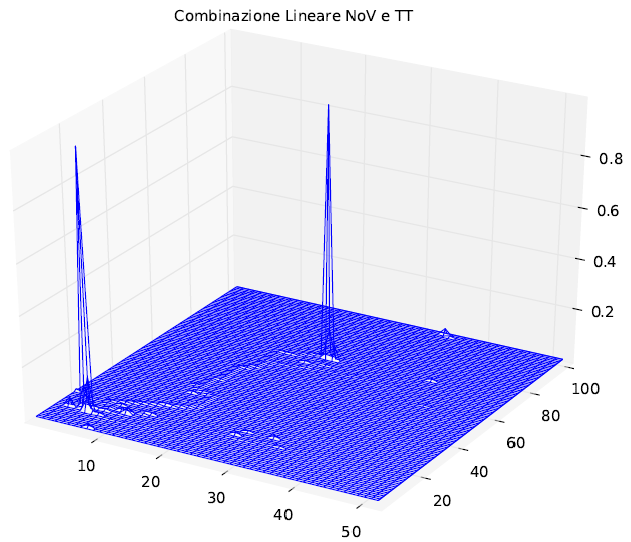
\includegraphics[scale=0.3]{Python/Python_Atlanta_CL.png}
    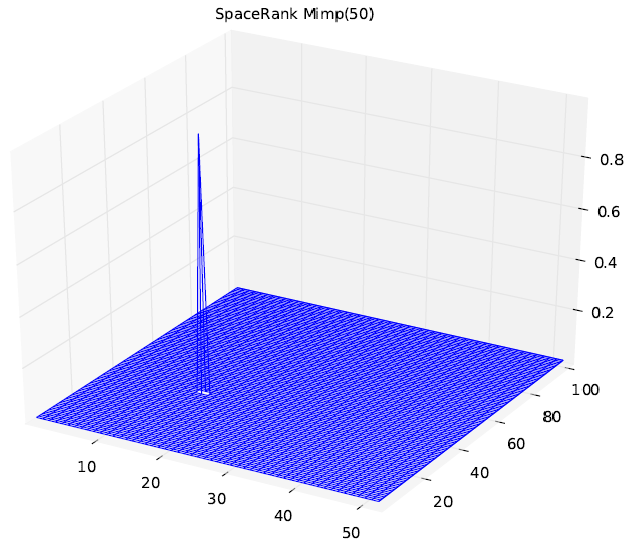
\includegraphics[scale=0.3]{Python/Python_Atlanta_SR.png}
    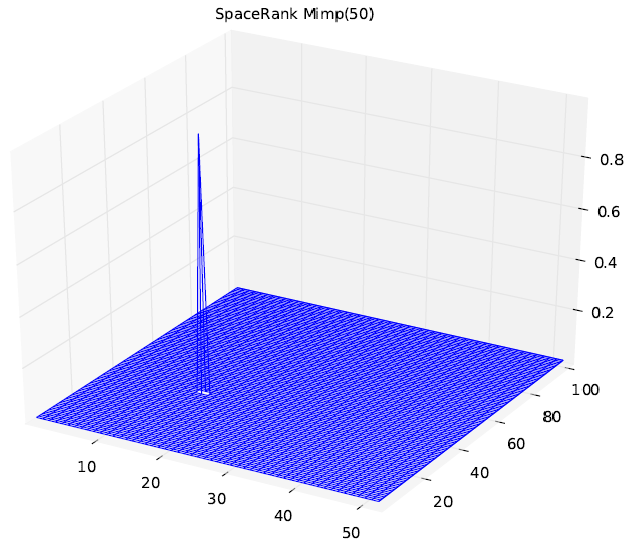
\includegraphics[scale=0.3]{Python/Python_Atlanta_SR.png}
    \caption[Arda 1]{Esempio di attrazione gravitazionale}
    \label{etichetta}
    \end{center}
\end{figure}


\section{ARDA}
\subsection{Dati Python}
\subsection{Dati Java}

\section{Valutazioni complessive}
Come gi\`a detto nell'introduzione e nel capitolo 2, le varie modifiche apportate
al codice hanno portato differenze marginali al livello di risultati complessivi.
Il limitato miglioramento \`e dovuto alla dimensione delle aree prese in esame, troppo
piccole per poter vedere i miglioramenti ottenibili delle nuove funzioni introdotte.\\
Questo per\`o non va incriminato alla scelta dei dati ma proprio alla natura dei
dati da analizzare, che cerca di prevedere le distanazioni su una serie di spostamenti
ottenuti monitorando degli utenti nelle loro spostamenti abituali. Ed \`e proprio la
natura ripetitiva dei spostamenti a rendere piccola la zona di interesse, visto che
difficilmente una persona compie spostamenti giornalieri su un'area di centinaia di
chilometri quadrati.
